\section{Super resolution} \label{sec:SR}

    Super resolution refers to an image processing technique looking to recover a corresponding high-resolution image from a low-resolution version of it, with applications that range from natural images \cite{zeyde2010single}, \cite{martin2001database} to satellite \cite{valsesia2021permutation} and medical imaging \cite{bashir2021comprehensive}. SR remains a challenging task in computer vision because it is considered an ill-posed problem: several HR images can generate exactly the same LR image. 

       \begin{figure}[H]
            \centering
            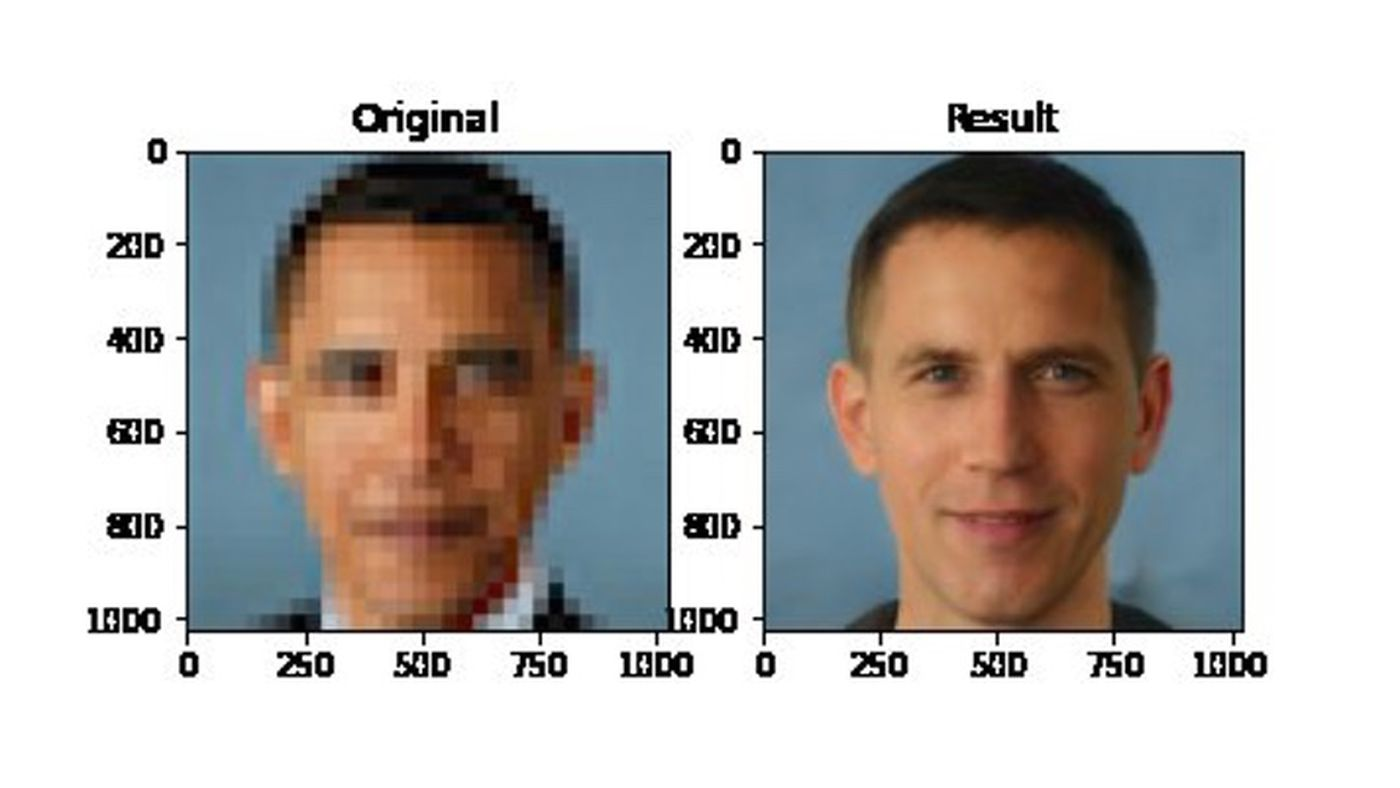
\includegraphics[width=\textwidth]{Includes/2-SR-ill-posed.jpg}
            \caption{Example of super resolution as an ill posed problem. A blurry picture of Barack Obama can be generated from an HR image of another person.}
            \label{fig:2-SR-ill-posed}
        \end{figure}
    
    Super resolution was first proposed in the 1960s, while the first use of multiple images dates of 1989. 
    Traditional interpolation-based methods for upsampling images were the first type of algorithms used for super resolution.
    The most common techniques are nearest-neighbor, bilinear and bicubic interpolation.
    Nearest-neighbor interpolation is the most straightforward algorithm, as the interpolated value is based on its nearest pixel values. 
    While this method requires almost no calculations, the results are usually blocky because there are no interpolated smooth transitions.
    Bilinear and bicubic interpolation produces smoother transitions using linear or cubic interpolation in both axes. 
    Bilinear interpolation needs a receptive fields of 2x2 and is usually faster, bicubic needs a receptive field of 4x4. 
    The latter is the most common baseline to quantify the improvement of any super resolution algorithm. 

    Machine learning was used for the first time in 2000. 
    Deep learning appears as a branch of machine learning, emphasizing the use of multi-layer neural network cascade for feature exctraction and representation. 
    The rise of the technology wave around 2010 changed the way of solving problems in different branches.
    Instead of piecing together individual feature extraction or functional modules to form a system, the focus is now to optimize parameters by global training after the whole system is designed, what is called end-to-end training.

    \begin{figure}[H]
        \centering
        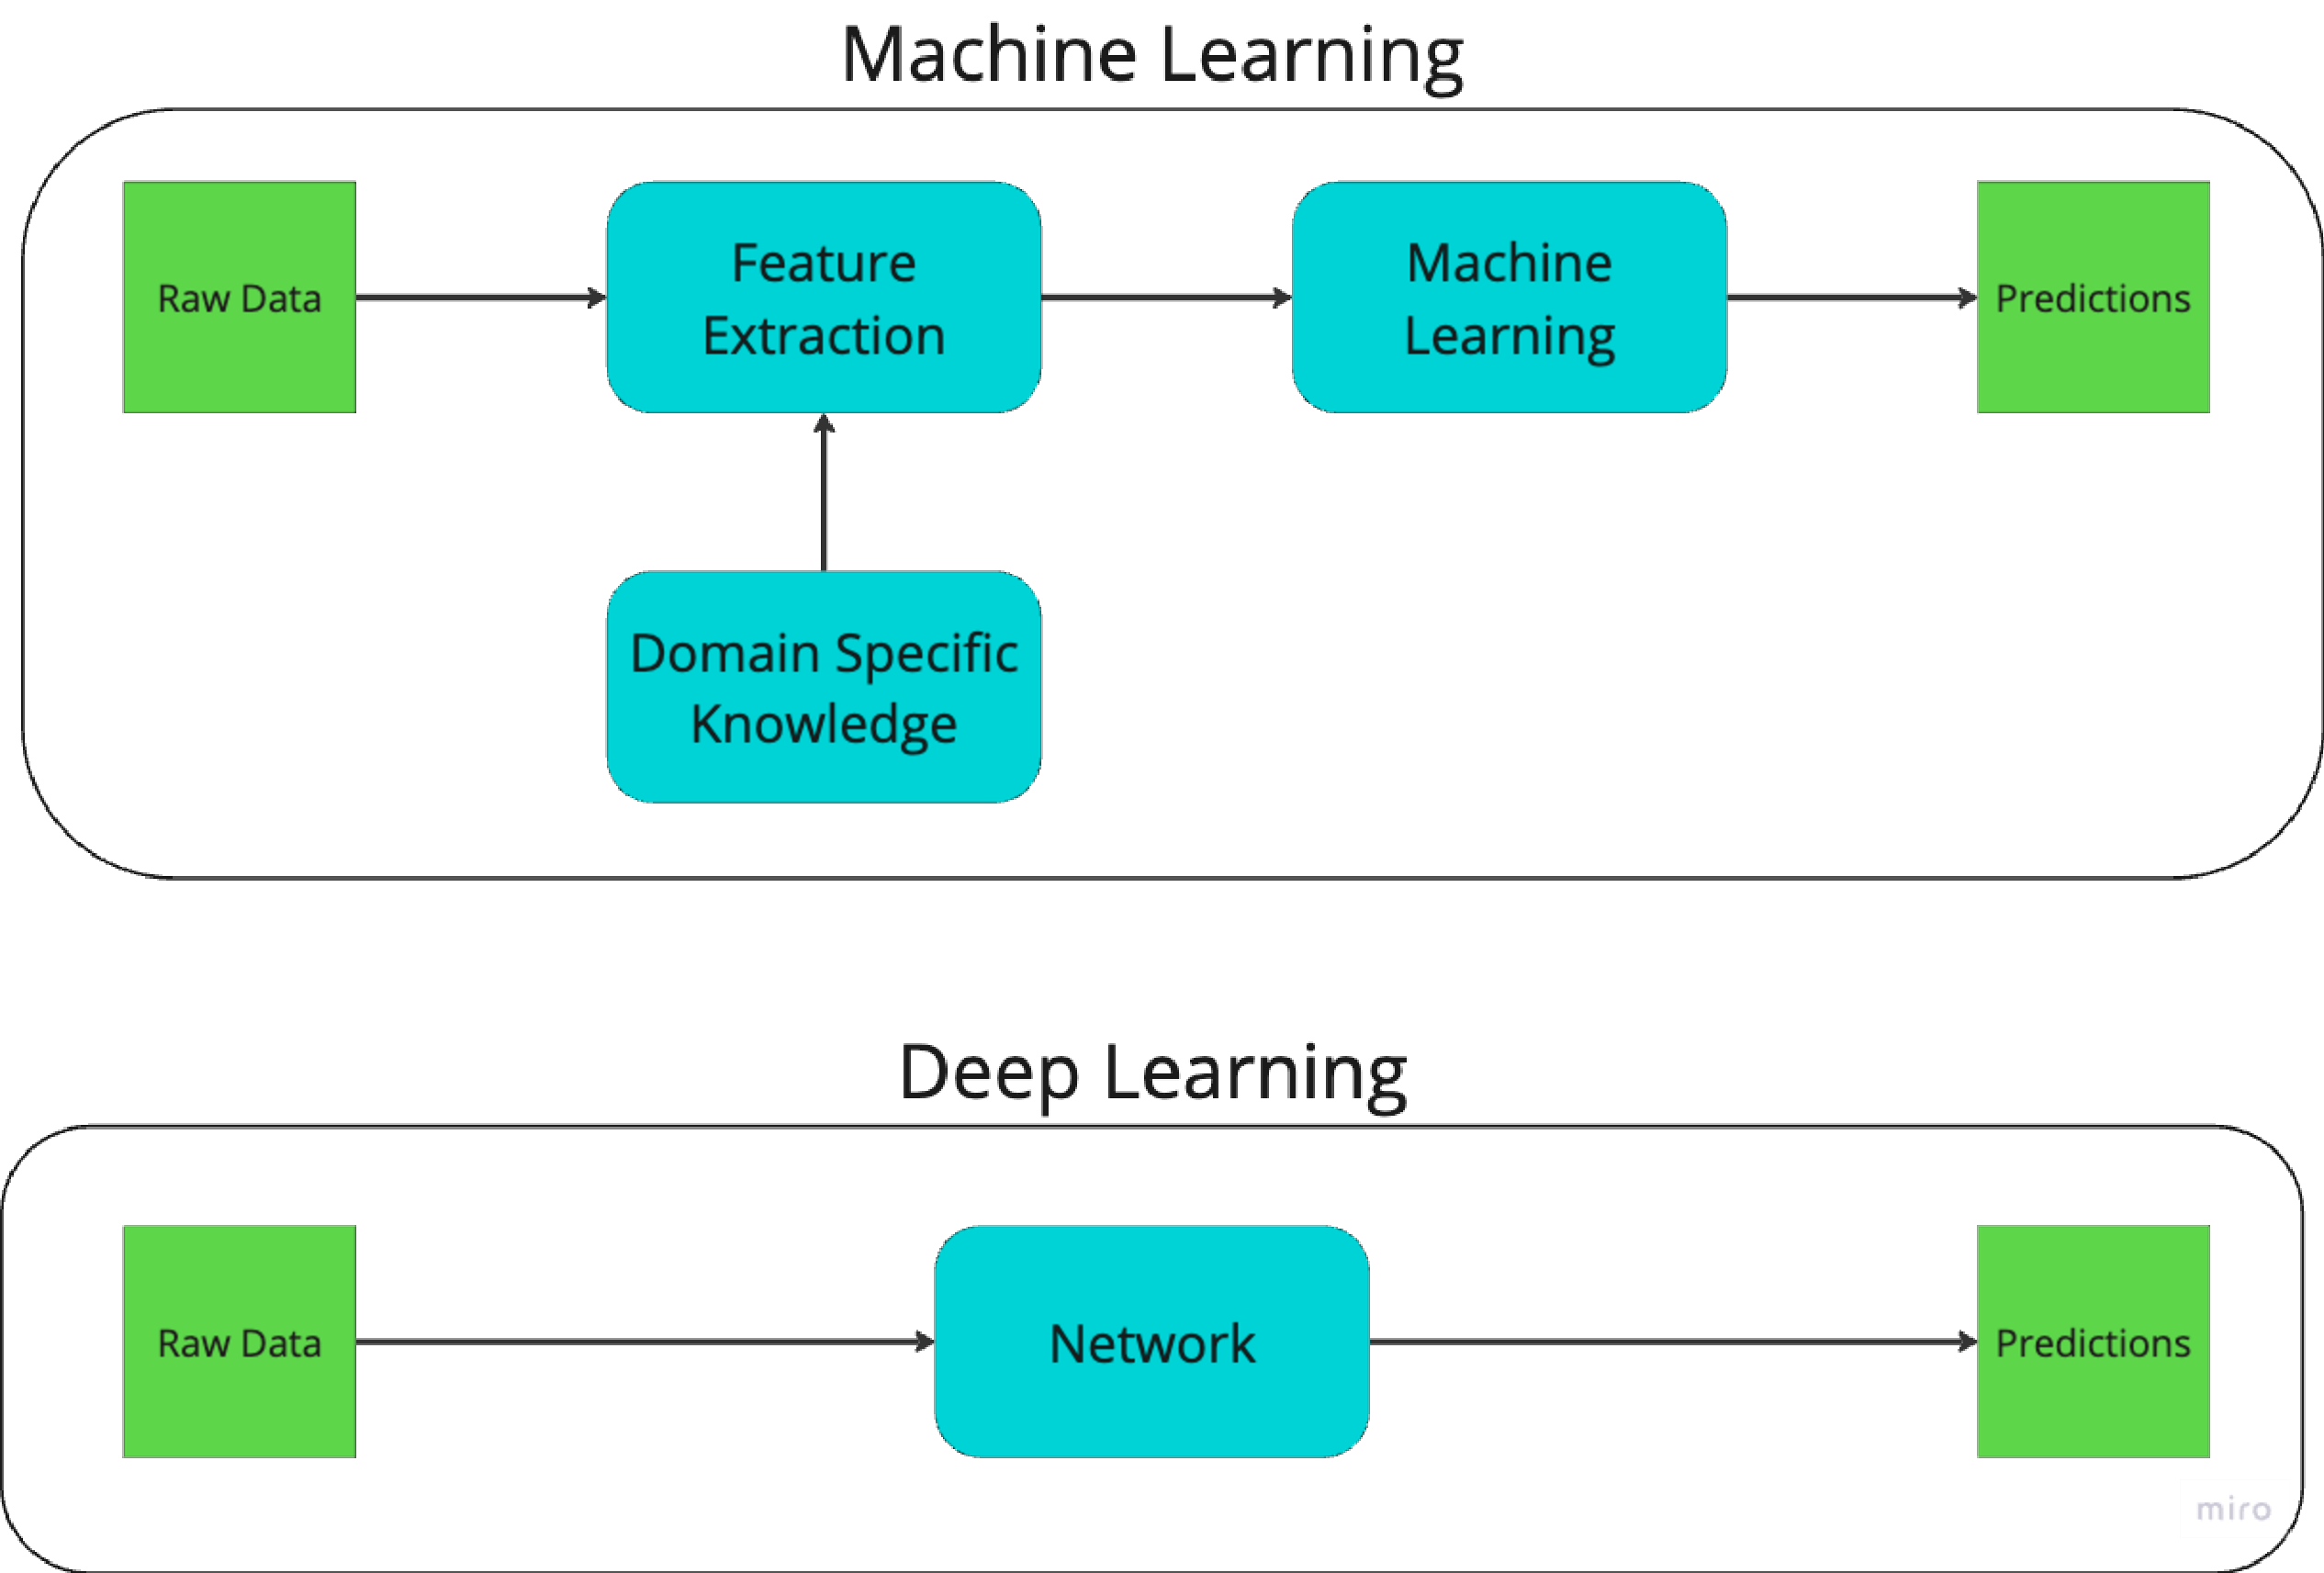
\includegraphics[width=\textwidth]{Includes/2-end-to-end-training.pdf}
        \caption{In traditional machine learning, the feature extraction step is crucial for performance, requiring a lot of domain knowledge. In deep learning, the feature extraction is learned from the data.}
        \label{fig:2-end-to-end-training}
    \end{figure}

    Super resolution using machine or deep learning is a supervised problem, meaning that the super resolved output must be compared to a HR ground truth image. 
    The difference between the two images is used to calculate the objective loss function that the model seeks to minimize.
    In very few occassions, paired LR-HR images are available.For that reason, the most common approach is to generate the LR images from the HR ground truth using a known degradation model, such as bicubic downsampling + white noise. An example of this method is depicted in Fig. \ref{fig:3-super-resolution-data}. 
    The real degradation process is unknown, and is affected by numerous factors such as sensor-induces noise, lossy compresion, speckle noise, motion blur and optical limitations, between others.
    The disadvantages of using such a simplified degradation process to generate a dataset will be further discussed throughout this work.

    \begin{figure}[H]
        \centering
        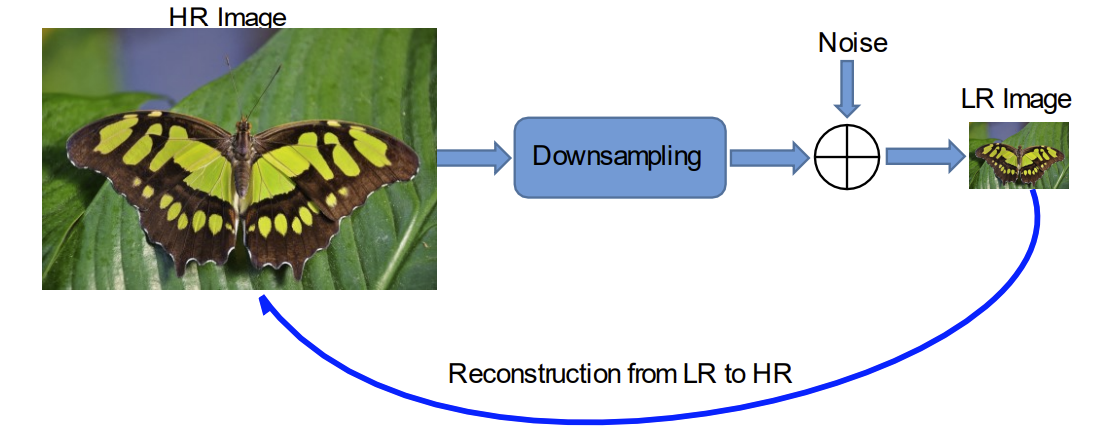
\includegraphics[width=\textwidth]{Includes/3-super-resolution-data.png}
        \caption{Example of generating a super resolution dataset, using a simplified known degradation model. Source: \cite{bashir2021comprehensive}.}
        \label{fig:3-super-resolution-data}
    \end{figure}

    

    \subsection{Single-Image Super Resolution}

        In a typical single-image super resolution (SISR) framework, the LR image $I^{LR}$ is modeled as follows:
    
        \begin{equation}
            I^{LR} = D(I^{HR},\Theta) = ( I^{HR} \ast k) \downarrow_s + \ n
            \label{eq:2-degradation-equation}
        \end{equation}
    
        Where $\Theta$ are the function parameters, $I^{HR} \ast k$ is the convolution between a blurring kernel $k$ and the unknown  HR image  $I^{HR}$, $\downarrow_s$ is the downsampling operator with scaling factor $s$ and $n$ is a noise term.
        The relationship between the LR and HR images $D$ is known as the degradation model.
        SISR objective is to solve the inverse equation and obtain $I^{HR}$ from $I^{LR}$, estimating $D^{-1}$ in the process. As stated before, this an extremely ill-posed problem as $D^{-1}$ is not injective, meaning there are infinite possibilities of $I^{HR}$ for which the equation condition hold. 

        A variety of deep learning methods were developed over the years to solve the SR problem, all of them are trained using both low and high-resolution images (LR-HR pairs), most of them generated as in Fig. \ref{fig:3-super-resolution-data}. The models can be classified based on the upsampling method chosen and it's location, the deep learning network and the loss used for learning.


        \subsubsection{Upsampling method}

        The upsampling is essential in deep learning-based SR methods. The most important feature of them is that, as opposed to traditional upsampling methods such as interpolation, they may add new information in the process.

        Sub-pixel convolutional layers performs upsampling by generating several additional channels using convolution, and by reshaping these channels, the resolution of the output is upsampled. The layer has a respective wide field that helps learn more contextual information that results in more realistic details, at the cost of possible artifacts. 

        Deconvolution layers do the inverse of the convolution operation. 
        That means predicting the probable HR image based on the feature maps from the LR image. The process consists on inserting zeros between the pixels of the LR image, and then applying a convolution operation. The amount of zeros is determined by the scaling factor. This method is widely used in SR methods due to its compatibility with the normal convolution, but may cause uneven overlapping in the generated HR image, resulting in a non-realistic image with decreased performance.


        The location of the upsampling layer plays an important role in the architecture. Pre-upsampling SR methods first upsample the LR image and then apply the convolutional layers. The convolutional network task is then to refine the already upsampled image. The biggest drawback is that the dimensions of the image is increzed at the beggining, resulting in higher computational and memory cost than other methods.
        Post-upsampling SR methods first apply the convolutional layers and then upsample the image. The convolutional network task is then to exctract features in a low-dimensional space. The computational cost is lower than pre-upsampling methods, but the extraction of the low level features for a good reconstruction may be more difficult than refining an already upsampled image. 
        This frameworks may be combined by iteratively up and downsampling the image \cite{timofte2015seven}, or by performing progressive upsampling until the desired dimensions are reached \cite{lai2017deep}.

        \subsubsection{Network design}

        In the last years, several deep learning network designs have been proposed to solve the SR problem.  The ones that are most interesting for this work due to their wide use in the literature are residual learning and attention-based learning. 
        
        Residual learning aims to mitigate the vanishing gradient problem that commonly occurs in deep neural network. This is done by adding a skip connection between the input and the output of the network that usually consists in convolutional, batch normalization and non-linear activation layers. This allows the learning of the difference between the input and the output. Mathematically, the residual learning can be formulated as follows:
        \begin{equation}
            F(x) = H(x) - x
            \label{eq:2-residual-learning}
        \end{equation}
        Where $H(x)$ is the mapping function of the network and $x$ is the input. If the residual is local, the skip connection is made over a small block of layers. Global residual makes the input and the output of the whole network to be correlated, which is a very desirable property in SR, as the HR image should have significant correlation with the LR image. In this case, the network transform the LR image into an HR image by generating the missing high-frequency details. 
        Attention learning is the idea where certain factors are given more preference. 

        In channel attention, a particular block is added in the model where global average pooling (GAP) squeezes the input channels; these constants are processed by two fully connected layers to generate channel-wise residuals that define how important is one pixel for each other.
        In SR, most of the models use local fields for the generation of SR pixels, while in a few cases, some textures or patches which are far apart are necessary for generating accurate local patches. This drives the development of attention blocks that extract non-local representations to add information of pixels that are far away from each other.


        \subsubsection{Loss functions}

        As in any supervised learning problem, the selection of the loss function is critical. In SR, they are used for measuring the error in the reconstruction of the HR image. 
        
        Initial research employed the loss at the fundamental block of an image, the pixel.
        The most common loss function is the Mean Squared Error (MSE), which is the average of the squared differences between the predicted and the ground truth images.
        The MSE is the most common loss function in image processing, but it is not the best choice for SR.
        This is because the MSE is very sensitive to outliers and tends to generate overly smooth results, as it converges to the mean of the distribution. Thus, researchers often have used L1 or MAE loss.
        These pixel losses focus on reconstruction fidelity and do not cater for the perceptual quality or textures of the image, resulting in less high-frequency details and overly smooth results. Other were designed to overcome this problem and will be discussed.

        If The perceptual quality is an important objective of the SR task, the differences between the generated and groud truth images could be assessed using an image classification network. The distance between the high-level data representation on a determined layer of the network for both images can be calculated in the following way:

        \begin{equation}
            \mathcal{L}(I^{\text{HR}}, I^{\text{SR}}; N) = \frac{1}{H*W*C}\sum_{i,j,k}(r^{l}_{i,j,k}(I^{\text{HR}}) - r^{l}_{i,j,k}(I^{\text{SR}}))^2
        \end{equation}

        Where $r^{l}$ is the output of the $k$-th channel of the $l$-th layer of the pre-trained classification network $N$ when the input is $I^{HR}$ or $I^{SR}$. $H$, $W$ and $C$ are the dimensions of the layer output (height, width and channels). 
        Commonly used classification networks are VGG \cite{simonyan2015deep} or ResNet \cite{he2015deep}.
        The purpose of the content los is to compare the information about image features from the network. This ensures the visual similarity between the original and generated image by comparing content and not individual pixels. Thus, content loss functions helps producing visually perceptible and more realistic loooking images and are widely used in SR \cite{ledig2017photorealistic,wang2018recovering}. On the other hand, this type of loss may not focus on the physical consistency of the image, resulting in possible artifacts that may look realistic but are non-existant. This is one of the main reasons why the content loss is not used in remote sensing applications.

        The adversarial loss is based on the generative adversarial network (GAN) \cite{goodfellow2014generative}. The GAN is composed of two networks, a generator and a discriminator. The generator is trained to generate SR images that are indistinguishable from the real HR images, while the discriminator is trained to distinguish between the generated and real images. 
        Training is performed in sequencial steps, where the generator is adjusted for better results that may fool the discriminator, and then the discriminator is adjusted to better distinguish between the generated and real images.
        When the generator is able to create outputs that conform to the distribution of the actual data, the discriminator is no longer able to distinguish between the generated and real images. In many cases, the mean squared error is used due to improved results: 

        \begin{equation}
            \begin{aligned}
            \mathcal{L}_{GANg}(I^{SR};D) &= (D(I^{SR}) - 1)^2 \\ 
            \mathcal{L}_{GANd}(I^{HR}, I^{SR};D) &= (D(I^{SR}))^2 + (D(I^{HR}) - 1)^2
            \end{aligned}
        \end{equation}

        Where $D$ is the discriminator network. 
        Results show that although the adversarial loss yielded lower physical consistency metrics, content and perceptual metrics were improved. 
        The use of the discriminator was able to regenerate intrincate patterns that were very difficult to learn using ordinary deep learning methods. 
        This is because the pixel-loss-based solutions perform a pixel-wise aggregation of the posible solutions in the pixel space, while adversarial loss drives the reconstruction towards the natural image manifold, producing more perceptually convincing solutions. 
        The main drawbacks of the adversarial loss are the inherent instability in the training of GANs and the probable degradation in physical consistency metrics.
        The latter is the main reason why this type of loss will not be used throughout this work.

        \begin{figure}[H]
            \centering
            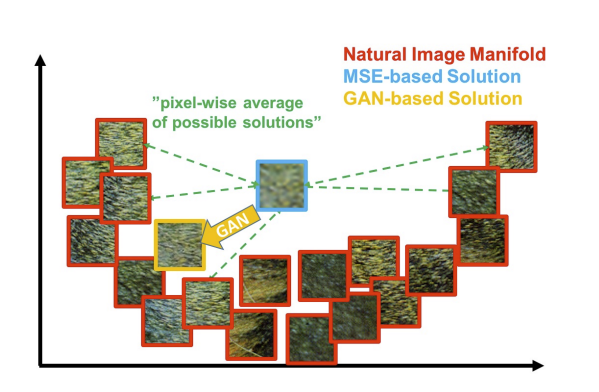
\includegraphics[width=\textwidth]{Includes/2-gans-natural-manifold.png}
            \caption{Illustration of patches from the natural image manifold and results coming from MSE pixel-loss (red) and GANs (orange). source:\cite{ledig2017photorealistic}}
            \label{fig:2-gans-natural-manifold}
        \end{figure}

















       




    \subsection{Multi-Image Super Resolution}

        Multi-Image Super-Resolution (MISR) is the task of yielding HR images by fusing multiple LR observations of the same scene, which allows the achievement of higher reconstruction accuracy than relying on only one image.
        The development of this approach progressed at a slower pace due to the extesive pre-processing requirements imposed on the input, as this algorithms have a high sensibility to the input variability and their proper co-registration.  

        When the input images are of the same nature, but taken at different points in the temporal dimension, the problem is often called multi-image super resolution.
        On the other hand, when the images are taken at the same time but they come from different sensors and show different spectral bands, it is called multi-spectral super resolution, which will be further discussed. 

        The main problem in MISR is the difficulty to generate a dataset with multiple images of the same scene, and it is the main reason why SISR is more popular.
        In 2019, the European Space Agency (ESA) organized an SR challenge  \cite{martens2019superresolution} based on real-world scenes acquired by the PROBA-V satellite, each of which contains an HR image (100m GSD) coupled with at least nine LR images that are not perfectly co-registered and they may be taken months apart. 
        This challenge, with a not-synthetically generated HR-LR image pairs, fostered a new generation of model architectures that are able to fuse the multiple LR images to create better reconstructions \cite{Salvetti_2020,Bordone_Molini_2020}.
         Both of the cited networks were tested in synthetically generated datasets throuhout this work and showed better performance than SISR networks, but they were discarded because of the impossibility to have a multi-image dataset using real FOREST-2 images.

        \begin{figure}[H]
            \centering
            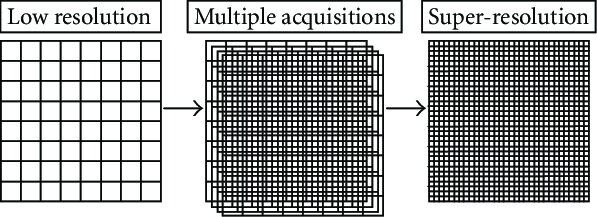
\includegraphics[width=\textwidth]{Includes/2-MISR.jpeg}
            \caption{Multi-image super resolution algorithms combine multiple low-resolution image acquisitions into a high-resolution image. Source: \cite{MISR2007}}
            \label{fig:2-MISR}
        \end{figure}
        
        \subsubsection{Multi-spectral super resolution}

        Also Referred to as "hyper-spectral super resolution" in the literature, The term "Multi-Spectral" emphasizes the use of multiple spectral bands, in contrast with the multi-image approach detailed previously. While the concept bears similarities to MISR, the key distinction lies in MSSR's use of a single scene captured with different spectral bands, as opposed to multiple images, to reconstruct a superior, super-resolved image.

        In the context of MSSR, each spectral band, corresponding to a specific wavelenght range, provides unique information about the observed scene. Some of the spectral bands yield better resolution because of their physical properties and the costs related to their sensors. Using this higher resolution bands to increase the detail in the lower bands seems like a resaonable approach.

        Traditional pan-sharpening algorithms could be considered as deterministic MSSR  algorithms. They are usually used to increase the resolution of a multi-spectral RGB image using the panchromatic band. The overlap between the wavelengths of the bands makes this algorithm straightforward and useful. However, it is ill-suited for Thermal Infrared (TIR) data due to the disjointed spectral domains of the visible and TIR bands.
        The result of pansharpening TIR data is shown in Fig. \ref{fig:2-pansharpening}  While the general resolution of the image is improved, several TIR hotspots are darkened and highlights from the visible bands are translated to the super-resolved image. This is particularly problematic for clouds, which have an inverse spectral response in the TIR and RGB bands. 
        
        \begin{figure}[H]
            \centering
            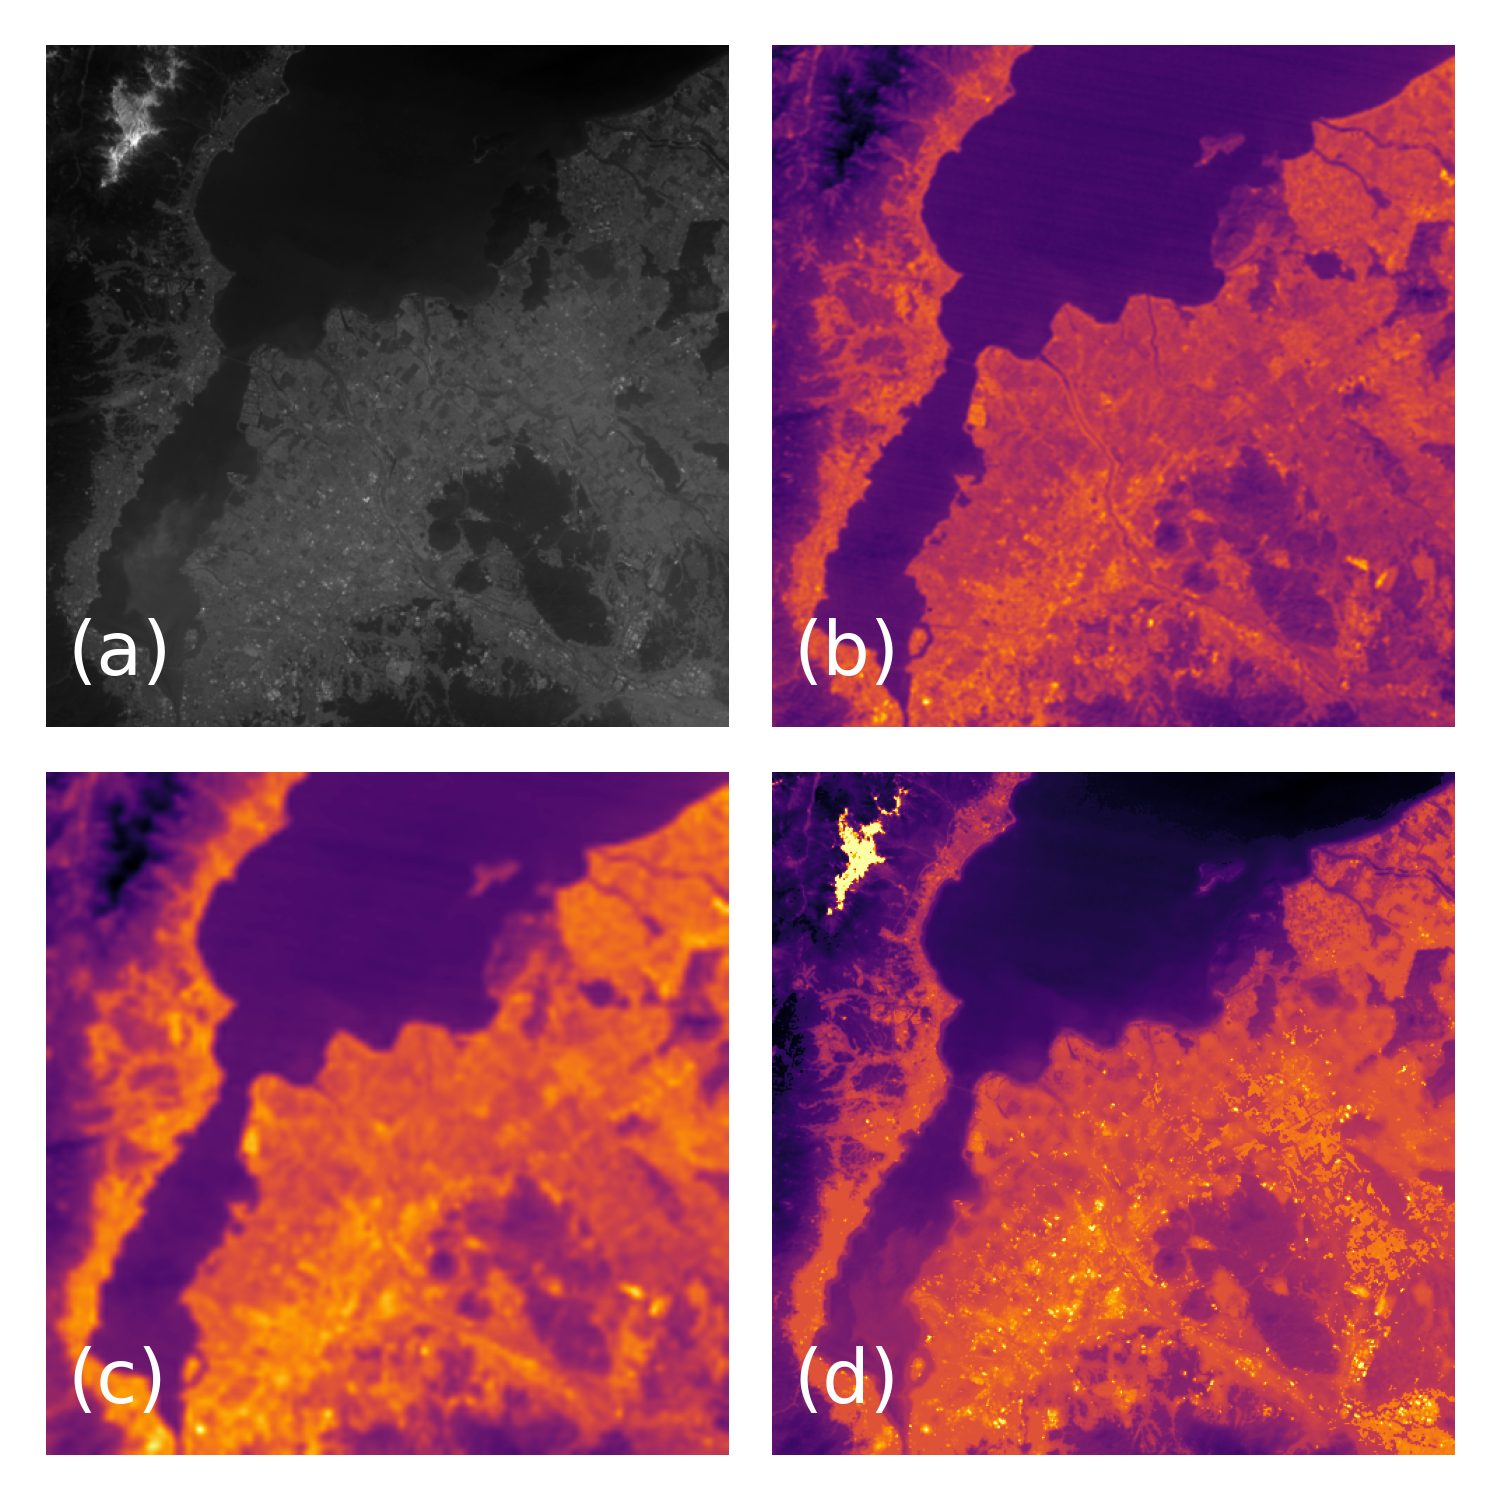
\includegraphics[width=\textwidth]{Includes/2-pansharpen.png}
            \caption{Example of Pan-sharpening on TIR data using a panchromatic band. (a) Panchromatic band, (b) HR TIR image, (c) Downsampled version of the TIR image , (d) Pansharpened image. 
            The pan-sharpened image is less blurry than the LR, but a lot of artifacts are produced, specially in clouds. Source: \cite{myself2023}}
            \label{fig:2-pansharpening}
        \end{figure}

        In \cite{myself2023}, A deep learning MSSR network is trained assuming the presence of common information between low-resolution LWIR images and their higher resolution RGB counterparts, with the objective of creating a super-resolved product in the LWIR band by an effective fusion. This improved image retains the essential thermal information, while simultaneously incorporates enhanced spatial resolution details captured from the visible bands. 
        MSSR remains a more promising alternative than MISR because it doesn't have the pre-processing burden that the latter has, as the images are well co-registered in the spatial and temporal domain.
        Additionally, most satellites have multi-spectral sensors, making the dataset generation much easier.

    \subsection{The domain gap problem} \label{subsec:domaingap}
 
        SR is a supervised problem, the super resolved image is compared to the HR ground truth and the differences (pixel-by-pixel or perceptual) drive the gradients of the neural network to minimize the loss, in a fully supervised manner. 
        The objective of this work is to increase the resolution of FOREST-2 images, but a high resolution version of FOREST-2 is not available. 
        The only alternative is to use scenes from other missions that have a higher resolution.

        Most of the research in the field of SR is conducted by artificially producing HR-LR pairs by downscaling the HR images with known kernels, as in Fig. \ref{fig:3-super-resolution-data}.
        However, this is rarely the case when using "non-ideal", real world images.
        In spite of their success on synthetic datasets, the poor generalization capacity of the trained SR networks limits their application in real scenarios, leading to blurry images and strange artifacts in the SR results \cite{lugmayr2020ntire}.

        The domain gap problem occurs when there are systematic discrepancies between data use for training and the real-world data. 
        This is described in Fig. \ref{fig:2-domain-gap}, where the HR image is processed through different known degradations. 
        If an SR model is trained using the left-most degradation, it will produce undesirable results if LR images generated by the other degradations are used as input.
        In this example, the left-most degradation seems to have better resolution and less noise than the rest. This will lead to noisier and blurrier results when using the other degradations as input.

        \begin{figure}[H]
            \centering
            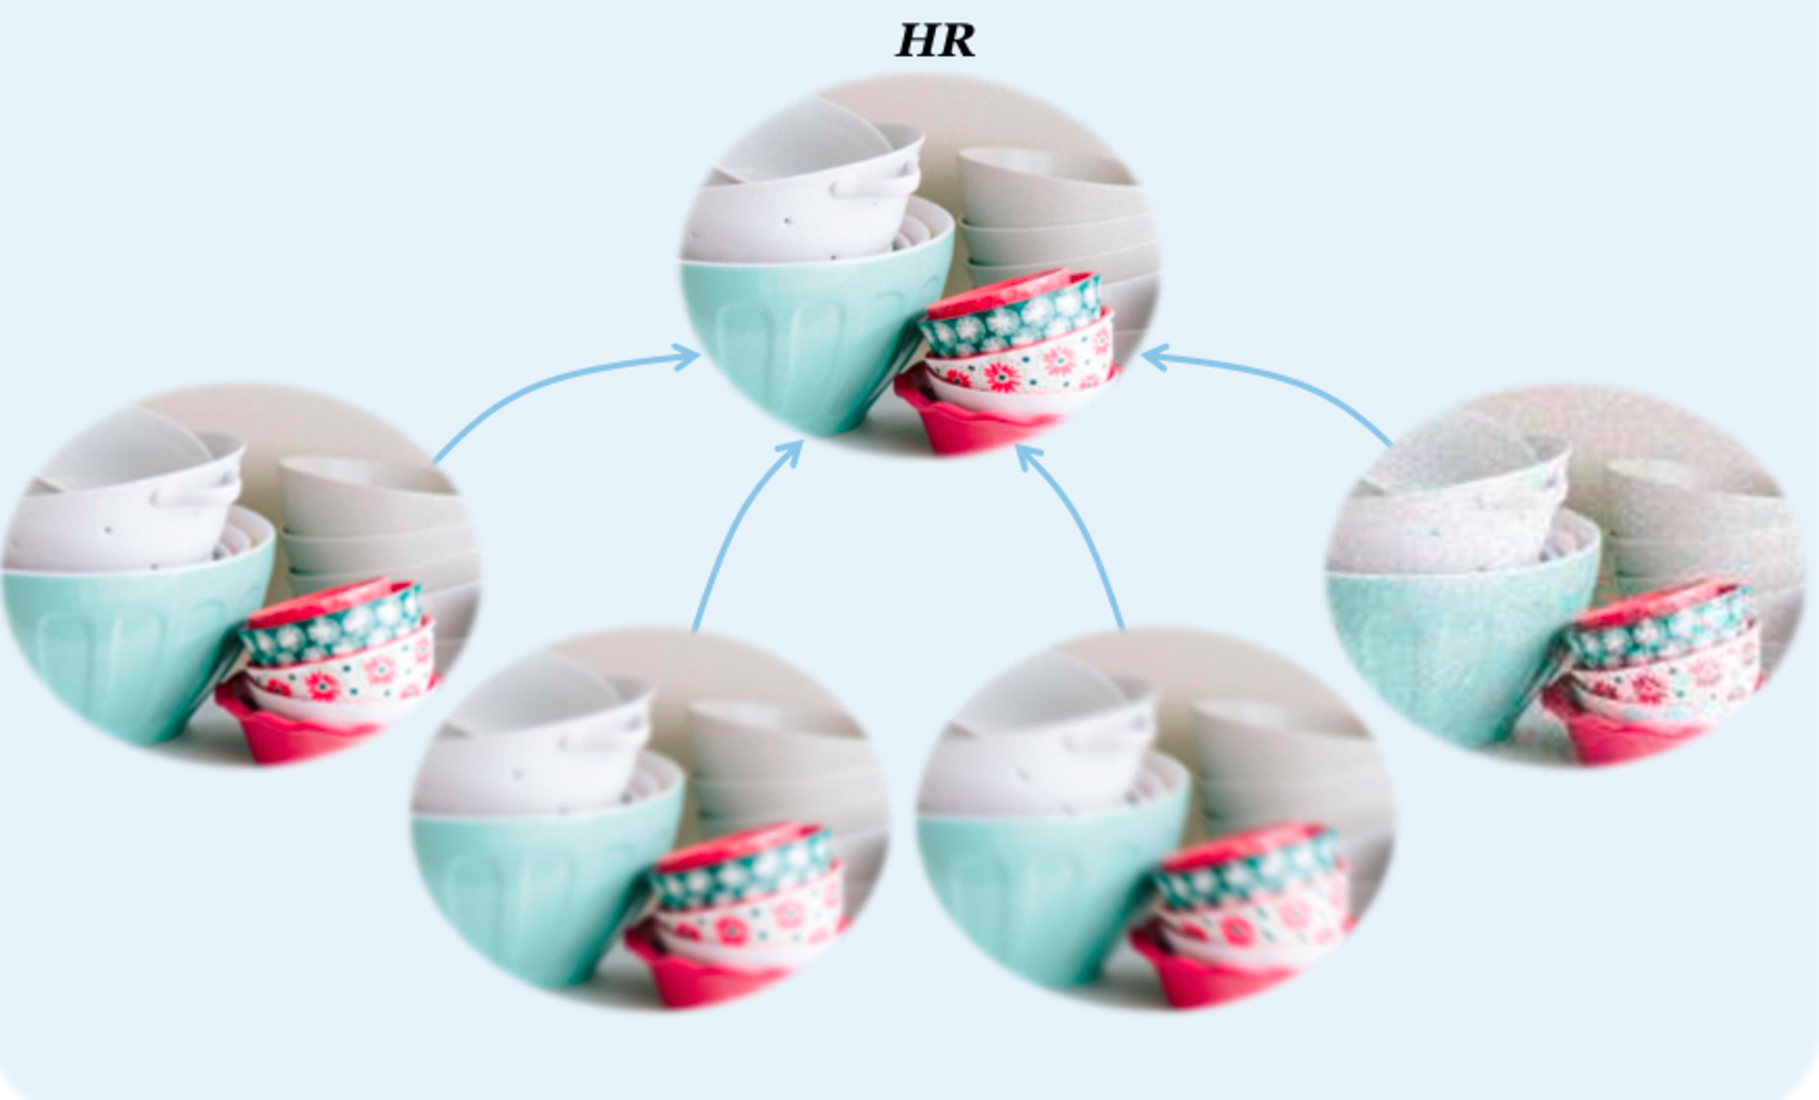
\includegraphics[scale=0.4]{Includes/2-domain-gap.pdf}
            \caption{Effects of different degradation models on one HR image. Source: \cite{liu2021blind}}
            \label{fig:2-domain-gap}
        \end{figure}

    \subsection{Blind image Super Resolution}

        The problem of SR with an unknown degradation process is known as blind SR. 
        Growing attention has been paid to blind SR in recent years, towards filling the domain gap presented in \ref{subsec:domaingap}.
        A schematic diagram of the problem is shown in Fig. \ref{fig:2-DomainGap}. 
        Non-blind SR methods assume that the degradation process is known, and maps the bicubic downsampled LR image to the natural HR image space.
        However, an arbitrary LR input image, as a scene captured by a satellite, is usually degraded by an unknown process, which is difficult to be modelled explicitly.
        The arbitrary LR input is not in the same domain as the bicubic downsamopled LR image, and thus the non-blind SR methods are not successful in the super resolution process.
        There will be a large domain gap between the SR output and the desired image samples from the target natural HR domain, leading to a poor-quality result.
        Blind SR methods, on the other hand, aim to learn the degradation process from the training data, and map the arbitrary LR input image to the natural HR image space.
        
        \begin{figure}[H]
            \centering
            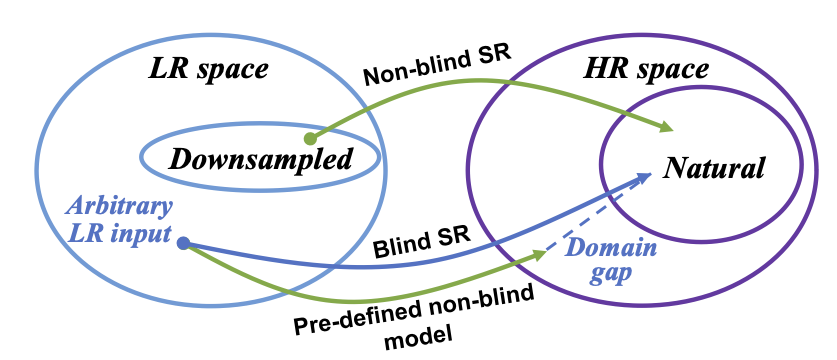
\includegraphics[width=\textwidth]{Includes/2-DomainGap.png}
            \caption{Domain interpretation of differences between non-blind and blind SR. Source: \cite{liu2021blind}}
            \label{fig:2-DomainGap}
        \end{figure}

        In the literature, two main approaches exist to bridge the gap: 
        Explicit modelling based on an extension of eq. \ref{eq:2-degradation-equation} and implicit modelling thought distribution learning of the degradation process.
        Explicit modelling can be further classified into two sub-categories according to whether they employ external datasets or rely on a single input image to solve the SR problem.


        \subsubsection{Explicit modelling with external dataset}

        This kind of methods use an external dataset to train an SR model well adapted to  variant blurring kernels and noises. 
        Typically, a traditional SISR is employed and an estimation of the kernel and the noise is used as a conditional input along with the LR image.
        After the training process, the model will be able to produce good results only in the now bigger pool of degradation types covered in the training dataset.
        According to whether the degradation is estimated or given, this approach can be further classified into two sub-categories.


        Explicit modelling without kernel estimation aims to directly concatenate a pre-defined degradation map to the LR input, as depicted in Fig \ref{fig:2-external-dataset-stretching}. 
        This allows feature adaptation according to the specific degradation model and helps to cover multiple degradation types during training. 
        The PCA technique used to project the degradation map can be replaced with a shallow neural network that may learn a kernel mapping that better fits the specific SR model used.

        \begin{figure}[H]
            \centering
            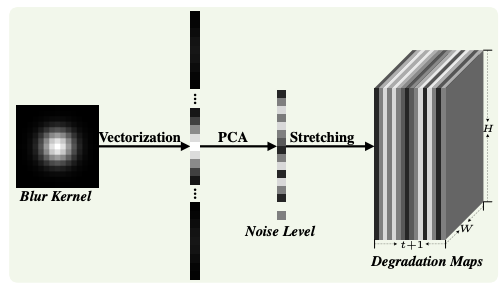
\includegraphics[width=\textwidth]{Includes/2-external-dataset-stretching.png}
            \caption{Dimensionality stretching strategy to concatenate the degradation map to the LR input. 
                     The vectorized kernel is projected onto a space of a lower dimensionality, and then stretched to generate $t$ feature maps with the same shape of the input image.
                     The noise level is also concatenated. Source: \cite{zhang2018residual} }    
            \label{fig:2-external-dataset-stretching}
        \end{figure}

        The biggest drawback  of this approach is that it relies on an additional input of degradation estimation, specially the kernel. 
        Howerver, estimating the correct kernel from an arbitrary LR image is not easy and kernel mismatch will result in a dramatic loss in SR performance.
        This method remains feasible only when a way of obtaining a reliable degradation estimation is available.
        Otherwise, a manual process to find the best input for better result is needed.
        
        Explicit modelling with kernel estimation aims to estimate the kernel from the LR input image in an iterative way until a good enough result is obtained \cite{gu2019blind}.
        The main idea is to take advantage of intermediate SR results because some of the artifacts caused by kernel mismatch show regular patterns that a corrector network can use to perfrom kernel correction.
        Methods like \cite{luo2020unfolding}, enhance the approach by unifying the kernel correction and SR network into an end-to-end trainable network. 
        However, the iterative nature of this method leads to higher inference time. Additionally, the optimal number of iterations is not known and must be determined empirically.

        Other approaches propose to learn a bling SR model by merely covering more degradations with more realistic kernels in the training dataset, creating a large pool.
        Kernels from this pool are used to synthetize the training pairs in a non-blind setting. 
        The more general training dataset enables the SR model to adapt to real input images. 
        However, it is very hard to cover all the possible degradation types in the real world, and the model will fail when facing a new degradation type.


        \subsubsection{Explicit modelling with single image}

        SR modelling with a single image is based on internal statistics of natural images: patches of a single image tend to recur within and across different scales of the image \cite{zontak2011}.
        This characteristic is very powerful, since it is image-specific and unsupervised. It was used first in 2009 in a method that does not used deep learning \cite{glasner2009}, and gained traction with KernelGAN \cite{bellkligler2020blind}. 
        KernelGAN interprets the maximization of patch recurrence as a data distribution learning problem, assuming that the downsampled version of an LR image generated by the optimal kernel should share the same patch distribution with the original LR input.
        Using a GAN framework, a deep linear network is used as a generator to parametrize the underlying SR kernel, and a discriminator distinguishes generated patches from those of the original LR image.
        Once training finishes, the output of the generator is an estimation of the blurring kernel of the input image. 

        \begin{figure}[H]
            \centering
            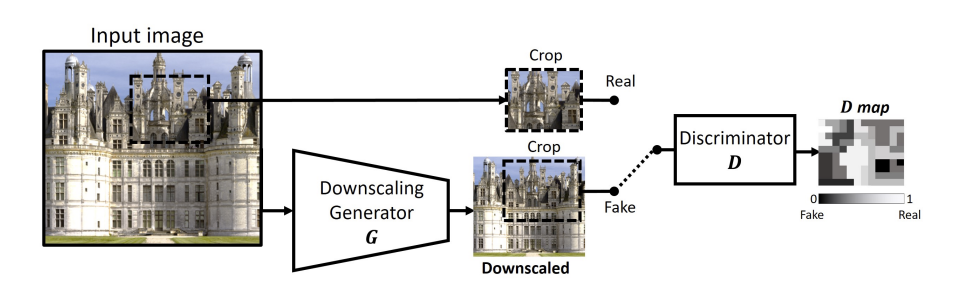
\includegraphics[width=\textwidth]{Includes/2-kernelGAN.png}
            \caption{KernelGAN schematic diagram. The discriminator tries to distinguish between the generated patches and the original LR image patches. G learns perform 2x downscaling while fooling the discriminator by maintaining the same distribution of patches. Source \cite{bellkligler2020blind}}    
            \label{fig:2-kernelGAN}
        \end{figure}

        This idea of self-supervision based on patch recurrence is also applied to perform SR without pre-training, as in zero-shot super resolution (ZSSR) \cite{shocher2017zeroshot}.
        In this case, the training is conducted using HR-LR pairs generated from a single LR image.
        The original input is regarded as HR and downsampled versions of it as LR using a kernel. 
        The network trained on these image pairs will be capable of inferring relationships across different scales which is then used to super-resolve the input.
        ZSSR is still not fully blind, it requires an estimated blur kernel as input. 
        For that reason, a joint framework that combines ZSSR and KernelGAN yields very good results.
        For a given image, KernelGAN estimates the blurring kernel that is then used in ZSSR to perform super resolution.

        While the idea of self-supervision is very flexible and efficient, its basic assumption may fail in certain cases.
        Hence, this approach can only produce favourable SR outputs for a limited set of images that have recurring contents across scales.



        \subsubsection{Implicit modelling} \label{subsubsec:implicit-modelling}

        Implicit modelling aims to grasp the underlying degradation model through learning from an external dataset.
        On paired HR-LR images, the SR model is already enough. However, these datasets are rarely available in real-world scenarios.
        Usually the data available is unpaired, meaning that HR images and LR images with realistic degradations are available, but there is no correspondence between them.
        Existing approaches exploit the data distribution learning ability of GANs, where discriminators are used to distinguish between the generated images from the real ones, pushing the generator towards an appropiate direction.
        
        First attempts for implicit modelling were based on CycleGANs \cite{CycleGAN2017}, that consists of two generators and two discriminators that move from domain A to B and viceversa. 
        The cycle consistency loss is based on the principle that after a round-trip transformation, the original image should be recovered.
        In CinCGAN \cite{yuan2018unsupervised}, the HR input is transformed using bicubic downsampling before doing SR with a pre-trained network and is regarded as the clean LR domain.
        Two CycleGAN structures are applied to transform the LR input to the clean LR domain and to the HR domain. 
        This way, no paired data is necessary.

        Another way of performing implicit modelling is using a single GAN to learn the degradation process from HR to LR, and generate a supervised paired dataset that can be used for training the SR network.
        The generator simulates the degradation from the HR domain to the LR domain and the discriminator distinguishes between the generated LR images and the real LR images.
        In these methods, such as \cite{luo2022learning,bulat2018learn}, usually the discriminator architecture is focused to distinguish the images using the high-frequency contents of them, due to the fact that degradations usually have a big overlap at lower frequencies.
        To further reduce the domain gap, several extensions of the method are proposed. 
        In \cite{wei2020unsupervised}, both the generated and real LR images are used to train the SR model.
        The super resolved version of the generated LR images can be compared with the original HR input using a pixel-wise loss, and the super resolved real LR images can be used for training trough a discriminator that distinguishes between them and the HR images.

        \begin{figure}[H]
            \centering
            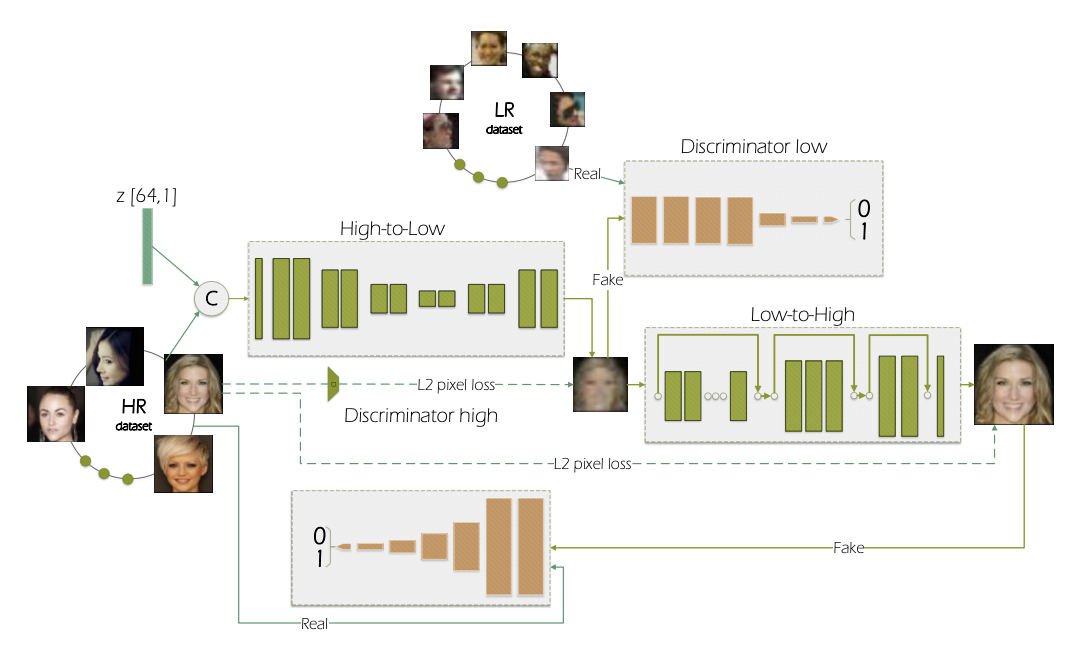
\includegraphics[width=\textwidth]{Includes/2-degradation-gan.png}
            \caption{Degradation GAN schematic diagram. The architecture includes one LR generator, on SR network and two discriminators. Source: \cite{bulat2018learn}.}    
            \label{fig:2-degradation-gan}
        \end{figure}
        
    
        While very flexible, limitations of implicit modelling are the dependency on huge dataset that is just not possible in some applications. 
        Additionally, several artifacts may be produced in the SR results due to the difficulty and instability of GANs training.
        The choice of the generator in the case of degradation learning GAN is also very important, if it is not well constrained enough, it will produce unrealistic results that will misguide the SR network and lead to poor results even after long training sessions.
         
         




        
























        
        
        

        

        

        










        

\clearpage